% answers.tex —— 2013 年·辽宁卷·理科 · 参考答案与详细解析片段
% 由 tools/generate_projects.py 依来源总账自 2013/2013_数学真题_辽宁理_试题.md + 2013/2013_数学真题_辽宁理_解析正文.md + 2013/2013_数学真题_辽宁理_答案要点.md 生成，勿手改（改源 MD 后重跑）


\begin{answer}
\gksolhead{1}{}

\textbf{题目}：

复数 $z=\dfrac{1}{\mathrm i-1}$ 的模为\mbox{（　　）}

（A）$\dfrac12$；（B）$\dfrac{\sqrt2}2$；（C）$\sqrt2$；（D）$2$。

\Needspace{4\baselineskip}
\textbf{解析}
\Needspace{5\baselineskip}
由复数模的性质，
\nopagebreak[4]
\[|z|=\left|\frac1{\mathrm i-1}\right|=\frac1{|\mathrm i-1|}=\frac1{\sqrt{0^2+(-1)^2}}=\frac1{\sqrt2}=\frac{\sqrt2}2.\]
选 B。

\gkanswer{答案：B。$|z|=\dfrac1{|\mathrm i-1|}=\dfrac1{\sqrt2}=\dfrac{\sqrt2}2$。}

\end{answer}
\begin{answer}
\gksolhead{2}{}

\textbf{题目}：

已知集合 $A=\{x\mid 0<\log_4x<1\}$，$B=\{x\mid x\leqslant2\}$，则 $A\cap B=$\mbox{（　　）}

（A）$(0,1)$；（B）$(0,2]$；（C）$(1,2)$；（D）$(1,2]$。

\Needspace{4\baselineskip}
\textbf{解析}
\Needspace{5\baselineskip}
由 $0<\log_4x<1$ 及对数函数的单调性，
\nopagebreak[4]
\[\log_41<\log_4x<\log_44,\]
\Needspace{5\baselineskip}
即
\nopagebreak[4]
\[1<x<4,\]
\Needspace{5\baselineskip}
所以 $A=(1,4)$。又 $B=(-\infty,2]$，故
\nopagebreak[4]
\[A\cap B=(1,2].\]
选 D。

\gkanswer{答案：D。$0<\log_4x<1$ 给出 $1<x<4$，与 $x\leqslant2$ 取交集得 $(1,2]$。}

\end{answer}
\begin{answer}
\gksolhead{3}{}

\textbf{题目}：

已知点 $A(1,3)$，$B(4,-1)$，则与向量 $\overrightarrow{AB}$ 同方向的单位向量为\mbox{（　　）}

（A）$\left(\dfrac35,-\dfrac45\right)$；（B）$\left(\dfrac45,-\dfrac35\right)$；（C）$\left(-\dfrac35,\dfrac45\right)$；（D）$\left(-\dfrac45,\dfrac35\right)$。

\Needspace{4\baselineskip}
\textbf{解析}
\nopagebreak[4]
\[\overrightarrow{AB}=(4-1,\,-1-3)=(3,-4),\]
\Needspace{5\baselineskip}
其模为
\nopagebreak[4]
\[|\overrightarrow{AB}|=\sqrt{3^2+(-4)^2}=5.\]
\Needspace{5\baselineskip}
与 $\overrightarrow{AB}$ 同方向的单位向量为
\nopagebreak[4]
\[\frac{\overrightarrow{AB}}{|\overrightarrow{AB}|}=\left(\frac35,-\frac45\right).\]
选 A。

\gkanswer{答案：A。$\overrightarrow{AB}=(3,-4)$，$|\overrightarrow{AB}|=5$，故单位向量为 $\left(\dfrac35,-\dfrac45\right)$。}

\end{answer}
\begin{answer}
\gksolhead{4}{}

\textbf{题目}：

下面是关于公差 $d>0$ 的等差数列 $\{a_n\}$ 的四个命题：

$p_1$：数列 $\{a_n\}$ 是递增数列；

$p_2$：数列 $\{na_n\}$ 是递增数列；

$p_3$：数列 $\left\{\dfrac{a_n}{n}\right\}$ 是递增数列；

$p_4$：数列 $\{a_n+3nd\}$ 是递增数列。

其中的真命题为\mbox{（　　）}

（A）$p_1$，$p_2$；（B）$p_3$，$p_4$；（C）$p_2$，$p_3$；（D）$p_1$，$p_4$。

\Needspace{4\baselineskip}
\textbf{解析}
设 $a_n=a_1+(n-1)d$，其中 $d>0$。

\begin{itemize}
\item $p_1$：$a_{n+1}-a_n=d>0$，故 $\{a_n\}$ 是递增数列，真命题；
\item $p_2$：$(n+1)a_{n+1}-na_n=a_1+2nd$，当 $a_1$ 充分小（例如 $a_1=-100$，$n=1$）时该差为负，故 $\{na_n\}$ 不一定是递增数列，假命题；
\item $p_3$：$\dfrac{a_n}{n}=d+\dfrac{a_1-d}{n}$，当 $a_1>d$ 时随 $n$ 增大而减小，故 $\left\{\dfrac{a_n}{n}\right\}$ 不一定是递增数列，假命题；
\item $p_4$：由 $a_{n+1}=a_n+d$，
\end{itemize}
\nopagebreak[4]
\[(a_{n+1}+3(n+1)d)-(a_n+3nd)=d+3d=4d>0,\]
故 $\{a_n+3nd\}$ 是递增数列，真命题。

真命题为 $p_1$，$p_4$。选 D。

\gkanswer{答案：D。$a_{n+1}-a_n=d>0$，且 $(a_{n+1}+3(n+1)d)-(a_n+3nd)=4d>0$，故 $p_1$，$p_4$ 真。}

\end{answer}
\begin{answer}
\gksolhead{5}{}

\textbf{题目}：

某班的全体学生参加英语测试，成绩的频率分布直方图如图所示，数据的分组依次为 $[20,40)$、$[40,60)$、$[60,80)$、$[80,100]$。若低于 $60$ 分的学生有 $15$ 人，则该班的学生人数是\mbox{（　　）}
\nopagebreak[4]
\begin{center}% 2013 年辽宁卷理科第 5 题：成绩频率分布直方图。
% 来源 PDF：普通高考/2013/2013辽宁理.pdf，第 1 页（印面 821）左栏。
% 分组 [20,40)、[40,60)、[60,80)、[80,100] 的柱高依次为
% 0.005、0.010、0.020、0.015（300 dpi 原页核对）。
\begin{tikzpicture}[font=\footnotesize, >=Stealth, line width=0.5pt,
  x=1.15cm, y=160cm]
  % 坐标轴：横轴以 20 分为一个单位
  \draw[->] (0,0) -- (5.75,0) node[right, yshift=-2pt] {成绩/分};
  \draw[->] (0,0) -- (0,0.0238);
  \node at (0,0.0295) {$\dfrac{\text{频率}}{\text{组距}}$};
  % 横轴刻度
  \foreach \x/\lab in {0/0,1/20,2/40,3/60,4/80,5/100}
    \draw (\x,0) -- (\x,-0.0006) node[below] {$\lab$};
  % 纵轴刻度与虚线
  \foreach \y/\lab in {0.005/0.005,0.010/0.010,0.015/0.015,0.020/0.020} {
    \draw (0,\y) -- (-0.08,\y) node[left] {$\lab$};
    \draw[dashed] (0,\y) -- (5.05,\y);
  }
  % 四个矩形位于 [20,40)、[40,60)、[60,80)、[80,100]，
  % 高度依次为 0.005、0.010、0.020、0.015
  \foreach \i/\h in {1/0.005,2/0.010,3/0.020,4/0.015} {
    \draw[fill=white] (\i,0) rectangle (\i+1,\h);
  }
\end{tikzpicture}
\end{center}
\nopagebreak[4]
（A）$45$；（B）$50$；（C）$55$；（D）$60$。

\Needspace{4\baselineskip}
\textbf{解析}
\Needspace{5\baselineskip}
组距均为 $20$，各组的频率等于“组距 $\times$ 频率/组距”。低于 $60$ 分的两组为 $[20,40)$ 与 $[40,60)$，由直方图读出其频率/组距分别为 $0.005$ 与 $0.010$，故低于 $60$ 分的频率为
\nopagebreak[4]
\[(0.005+0.010)\times20=0.30.\]
\Needspace{5\baselineskip}
设该班学生人数为 $n$，则
\nopagebreak[4]
\[0.30n=15,\]
\Needspace{5\baselineskip}
解得
\nopagebreak[4]
\[n=50.\]
选 B。

\gkanswer{答案：B。低于 $60$ 分的频率为 $(0.005+0.010)\times20=0.30$，故人数为 $15\div0.30=50$。}

\end{answer}
\begin{answer}
\gksolhead{6}{}

\textbf{题目}：

在 $\triangle ABC$ 中，内角 $A$，$B$，$C$ 所对的边分别为 $a$，$b$，$c$，若 $a\sin B\cos C+c\sin B\cos A=\dfrac12b$，且 $a>b$，则 $\angle B=$\mbox{（　　）}

（A）$\dfrac{\pi}6$；（B）$\dfrac{\pi}3$；（C）$\dfrac{2\pi}3$；（D）$\dfrac{5\pi}6$。

\Needspace{4\baselineskip}
\textbf{解析}
\Needspace{5\baselineskip}
由正弦定理 $a=2R\sin A$，$b=2R\sin B$，$c=2R\sin C$，得
\nopagebreak[4]
\[a\cos C+c\cos A=2R(\sin A\cos C+\sin C\cos A)=2R\sin(A+C)=2R\sin B=b.\]
\Needspace{5\baselineskip}
代入已知等式：
\nopagebreak[4]
\[\sin B(a\cos C+c\cos A)=\frac12b,\]
\Needspace{5\baselineskip}
即
\nopagebreak[4]
\[\sin B\cdot b=\frac12b.\]
\Needspace{5\baselineskip}
因为 $b>0$，所以
\nopagebreak[4]
\[\sin B=\frac12.\]
\Needspace{5\baselineskip}
于是 $B=\dfrac{\pi}6$ 或 $B=\dfrac{5\pi}6$。若 $B=\dfrac{5\pi}6$，则由 $a>b$ 得 $A>B=\dfrac{5\pi}6$，从而 $A+B>\pi$，矛盾。故
\nopagebreak[4]
\[B=\frac{\pi}6.\]
选 A。

\gkanswer{答案：A。由射影定理 $a\cos C+c\cos A=b$，代入得 $\sin B=\dfrac12$；又 $a>b$ 排除 $B=\dfrac{5\pi}6$，故 $B=\dfrac{\pi}6$。}

\end{answer}
\begin{answer}
\gksolhead{7}{}

\textbf{题目}：

使 $\left(3x+\dfrac{1}{x\sqrt{x}}\right)^n$（$n\in\mathbf N_+$）的展开式中含有常数项的最小的 $n$ 为\mbox{（　　）}

（A）$4$；（B）$5$；（C）$6$；（D）$7$。

\Needspace{4\baselineskip}
\textbf{解析}
\nopagebreak[4]
\[\left(3x+\frac1{x\sqrt x}\right)^n=\left(3x+x^{-3/2}\right)^n.\]
\Needspace{5\baselineskip}
展开式的第 $k+1$ 项为
\nopagebreak[4]
\[T_{k+1}=\mathrm C_n^k(3x)^{n-k}\left(x^{-3/2}\right)^k
=\mathrm C_n^k3^{n-k}x^{n-\frac52k}.\]
\Needspace{5\baselineskip}
含有常数项，即存在整数 $k$（$0\leqslant k\leqslant n$）使
\nopagebreak[4]
\[n-\frac52k=0,\]
\Needspace{5\baselineskip}
亦即
\nopagebreak[4]
\[2n=5k.\]
所以 $n$ 必须是 $5$ 的倍数。又 $n\in\mathbf N_+$，最小的 $n=5$，此时 $k=2$，确实产生常数项。选 B。

\gkanswer{答案：B。通项中 $x$ 的指数为 $n-\dfrac52k$，常数项要求 $2n=5k$，最小的 $n=5$（此时 $k=2$）。}

\end{answer}
\begin{answer}
\gksolhead{8}{}

\textbf{题目}：

执行如图所示的程序框图，若输入 $n=10$，则输出 $S=$\mbox{（　　）}
\nopagebreak[4]
\begin{center}% 2013 年辽宁卷理科第 8 题：程序框图。
% 来源 PDF：普通高考/2013/2013辽宁理.pdf，第 1 页（印面 821）中栏。
% 流程：开始 → 输入 n → S=0,i=2 → i≤n? 是：S=S+1/(i^2−1)，i=i+2，回到判断；
% 否：输出 S → 结束。
\begin{tikzpicture}[font=\footnotesize, >=Stealth, line width=0.45pt,
  node distance=5mm,
  term/.style={draw, rounded corners=6pt, minimum height=1.8em, inner xsep=9pt},
  io/.style={draw, trapezium, trapezium left angle=70, trapezium right angle=110,
             minimum height=1.8em, inner xsep=6pt},
  box/.style={draw, minimum height=1.9em, inner xsep=6pt},
  dec/.style={draw, diamond, aspect=2.2, inner sep=1pt}]
  \node[term] (start) {开始};
  \node[io, below=5mm of start] (input) {输入 $n$};
  \node[box, below=5mm of input] (init) {$S=0$，$i=2$};
  \node[dec, below=6mm of init] (cond) {$i\leqslant n$};
  \node[box, below=7mm of cond] (acc) {$S=S+\dfrac{1}{i^2-1}$};
  \node[box, below=5mm of acc] (inc) {$i=i+2$};
  \node[io, right=15mm of cond] (output) {输出 $S$};
  \node[term, below=6mm of output] (end) {结束};
  \draw[->] (start) -- (input);
  \draw[->] (input) -- (init);
  \draw[->] (init) -- (cond);
  \draw[->] (cond) -- node[right] {是} (acc);
  \draw[->] (acc) -- (inc);
  \draw[->] (cond) -- node[above] {否} (output);
  \draw[->] (output) -- (end);
  % 循环支路：从 i=i+2 左侧引出，向上回到判断框入口
  \draw[->] (inc.west) -- ++(-1.45,0) |- (cond.west);
\end{tikzpicture}
\end{center}
\nopagebreak[4]
（A）$\dfrac5{11}$；（B）$\dfrac{10}{11}$；（C）$\dfrac{36}{55}$；（D）$\dfrac{72}{55}$。

\Needspace{4\baselineskip}
\textbf{解析}
\Needspace{5\baselineskip}
程序框图的循环体在 $i=2,4,6,8,10$ 时依次执行，故
\nopagebreak[4]
\[S=\sum_{i=2,4,6,8,10}\frac1{i^2-1}.\]
\Needspace{5\baselineskip}
利用
\nopagebreak[4]
\[\frac1{i^2-1}=\frac1{(i-1)(i+1)}=\frac12\left(\frac1{i-1}-\frac1{i+1}\right),\]
\Needspace{5\baselineskip}
得
\nopagebreak[4]
\[\begin{aligned}
S&=\frac12\left[\left(1-\frac13\right)+\left(\frac13-\frac15\right)+\left(\frac15-\frac17\right)
+\left(\frac17-\frac19\right)+\left(\frac19-\frac1{11}\right)\right]\\
&=\frac12\left(1-\frac1{11}\right)=\frac12\cdot\frac{10}{11}=\frac5{11}.
\end{aligned}\]
选 A。

\gkanswer{答案：A。$S=\displaystyle\sum_{i=2,4,\ldots,10}\frac1{i^2-1}=\frac12\left(1-\frac1{11}\right)=\frac5{11}$。}

\end{answer}
\begin{answer}
\gksolhead{9}{}

\textbf{题目}：

已知点 $O(0,0)$，$A(0,b)$，$B(a,a^3)$。若 $\triangle OAB$ 为直角三角形，则必有\mbox{（　　）}

（A）$b=a^3$；（B）$b=a^3+\dfrac1a$；（C）$(b-a^3)\left(b-a^3-\dfrac1a\right)=0$；（D）$|b-a^3|+\left|b-a^3-\dfrac1a\right|=0$。

\Needspace{4\baselineskip}
\textbf{解析}
\Needspace{5\baselineskip}
若 $a=0$，则 $B=(0,0)=O$；若 $b=0$，则 $A=(0,0)=O$，均不能构成三角形，故 $a\neq0$，$b\neq0$。于是
\nopagebreak[4]
\[\overrightarrow{OA}=(0,b),\qquad \overrightarrow{OB}=(a,a^3),\qquad \overrightarrow{AB}=(a,a^3-b).\]

\begin{itemize}
\item 若直角在 $O$，则 $\overrightarrow{OA}\cdot\overrightarrow{OB}=ba^3=0$，与 $a\neq0$，$b\neq0$ 矛盾，故不可能；
\item 若直角在 $A$，则
\end{itemize}
\nopagebreak[4]
\[\overrightarrow{AO}\cdot\overrightarrow{AB}=(0,-b)\cdot(a,a^3-b)=-b(a^3-b)=0,\]
\Needspace{5\baselineskip}
由 $b\neq0$ 得
\nopagebreak[4]
\[b=a^3;\]
\begin{itemize}
\item 若直角在 $B$，则
\end{itemize}
\nopagebreak[4]
\[\overrightarrow{BO}\cdot\overrightarrow{BA}=(-a,-a^3)\cdot(-a,b-a^3)=a^2-a^3(b-a^3)=a^2\left[1-a(b-a^3)\right]=0,\]
\Needspace{5\baselineskip}
由 $a\neq0$ 得
\nopagebreak[4]
\[b-a^3=\frac1a.\]

\Needspace{5\baselineskip}
因此 $\triangle OAB$ 为直角三角形必有
\nopagebreak[4]
\[(b-a^3)\left(b-a^3-\frac1a\right)=0.\]
选 C。

\gkanswer{答案：C。直角只能在 $A$ 或 $B$：在 $A$ 时 $b=a^3$，在 $B$ 时 $b=a^3+\dfrac1a$，故两因式之积为 $0$。}

\end{answer}
\begin{answer}
\gksolhead{10}{}

\textbf{题目}：

已知直三棱柱 $ABC-A_1B_1C_1$ 的 $6$ 个顶点都在球 $O$ 的球面上。若 $AB=3$，$AC=4$，$AB\perp AC$，$AA_1=12$，则球 $O$ 的半径为\mbox{（　　）}

（A）$\dfrac{3\sqrt{17}}2$；（B）$2\sqrt{10}$；（C）$\dfrac{13}2$；（D）$3\sqrt{10}$。

\Needspace{4\baselineskip}
\textbf{解析}
\Needspace{5\baselineskip}
底面 $\triangle ABC$ 中 $AB\perp AC$，$AB=3$，$AC=4$，故斜边
\nopagebreak[4]
\[BC=\sqrt{3^2+4^2}=5,\]
底面外接圆半径为 $\dfrac52$。

\Needspace{5\baselineskip}
直三棱柱的外接球球心是上、下底面外心连线的中点，球心到底面的距离为 $\dfrac{AA_1}2=6$。设球半径为 $R$，则
\nopagebreak[4]
\[R^2=\left(\frac52\right)^2+6^2=\frac{25}4+36=\frac{169}4,\]
\Needspace{5\baselineskip}
所以
\nopagebreak[4]
\[R=\frac{13}2.\]
选 C。

\gkanswer{答案：C。底面直角三角形斜边 $BC=5$，球心在上下底面外心连线的中点，$R^2=\left(\dfrac52\right)^2+6^2=\dfrac{169}4$，故 $R=\dfrac{13}2$。}

\end{answer}
\begin{answer}
\gksolhead{11}{}

\textbf{题目}：

已知函数 $f(x)=x^2-2(a+2)x+a^2$，$g(x)=-x^2+2(a-2)x-a^2+8$，设 $H_1(x)=\max\{f(x),g(x)\}$，$H_2(x)=\min\{f(x),g(x)\}$（$\max\{p,q\}$ 表示 $p$，$q$ 中的较大值，$\min\{p,q\}$ 表示 $p$，$q$ 中的较小值）。记 $H_1(x)$ 的最小值为 $A$，$H_2(x)$ 的最大值为 $B$，则 $A-B=$\mbox{（　　）}

（A）$16$；（B）$-16$；（C）$a^2-2a-16$；（D）$a^2+2a-16$。

\Needspace{4\baselineskip}
\textbf{解析}
\Needspace{5\baselineskip}
配方得
\nopagebreak[4]
\[f(x)=(x-a-2)^2-4a-4,\qquad g(x)=-(x-a+2)^2+12-4a.\]
\Needspace{5\baselineskip}
两式相减：
\nopagebreak[4]
\[f(x)-g(x)=2x^2-4ax+2a^2-8=2\left[(x-a)^2-4\right].\]
\Needspace{5\baselineskip}
因此
\nopagebreak[4]
\[f(x)\geqslant g(x)\iff |x-a|\geqslant2.\]
\Needspace{5\baselineskip}
当 $|x-a|\leqslant2$ 时，$f\leqslant g$，故
\nopagebreak[4]
\[H_1=g,\qquad H_2=f;\]
\Needspace{5\baselineskip}
当 $|x-a|\geqslant2$ 时，$f\geqslant g$，故
\nopagebreak[4]
\[H_1=f,\qquad H_2=g.\]

\Needspace{5\baselineskip}
先求 $A=\min H_1$。在 $|x-a|\leqslant2$ 上 $g$ 是开口向下的二次函数，最小值在端点取得；在端点 $x=a\pm2$ 处 $f=g$，且
\nopagebreak[4]
\[f(a-2)=12-4a,\qquad f(a+2)=-4a-4.\]
\Needspace{5\baselineskip}
在 $|x-a|\geqslant2$ 上 $H_1=f$，其最小值也在端点取得。故
\nopagebreak[4]
\[A=\min\{12-4a,\,-4a-4\}=-4a-4.\]

\Needspace{5\baselineskip}
再求 $B=\max H_2$。在 $|x-a|\leqslant2$ 上 $H_2=f$，最大值在端点取得，为
\nopagebreak[4]
\[\max\{12-4a,\,-4a-4\}=12-4a;\]
\Needspace{5\baselineskip}
在 $|x-a|\geqslant2$ 上 $H_2=g$，而 $g$ 的全局最大值 $12-4a$ 在 $x=a-2$ 处取得，该点属于边界。故
\nopagebreak[4]
\[B=12-4a.\]
\Needspace{5\baselineskip}
于是
\nopagebreak[4]
\[A-B=(-4a-4)-(12-4a)=-16.\]
选 B。

\gkanswer{答案：B。$A=-4a-4$，$B=12-4a$，故 $A-B=-16$。}

\end{answer}
\begin{answer}
\gksolhead{12}{}

\textbf{题目}：

设函数 $f(x)$ 满足 $x^2f'(x)+2xf(x)=\dfrac{\mathrm e^x}{x}$，$f(2)=\dfrac{\mathrm e^2}8$，则 $x>0$ 时，$f(x)$\mbox{（　　）}

（A）有极大值，无极小值；（B）有极小值，无极大值；（C）既有极大值又有极小值；（D）既无极大值也无极小值。

\Needspace{4\baselineskip}
\textbf{解析}
\Needspace{5\baselineskip}
令
\nopagebreak[4]
\[F(x)=x^2f(x).\]
\Needspace{5\baselineskip}
则
\nopagebreak[4]
\[F'(x)=x^2f'(x)+2xf(x)=\frac{\mathrm e^x}{x}.\]
\Needspace{5\baselineskip}
于是
\nopagebreak[4]
\[f(x)=\frac{F(x)}{x^2},\]
\Needspace{5\baselineskip}
且
\nopagebreak[4]
\[f'(x)=\frac{xF'(x)-2F(x)}{x^3}
=\frac{\mathrm e^x-2F(x)}{x^3}.\]
\Needspace{5\baselineskip}
再令
\nopagebreak[4]
\[G(x)=2F(x)-\mathrm e^x,\]
\Needspace{5\baselineskip}
则
\nopagebreak[4]
\[G'(x)=2\cdot\frac{\mathrm e^x}{x}-\mathrm e^x=\mathrm e^x\left(\frac2x-1\right).\]
\Needspace{5\baselineskip}
当 $0<x<2$ 时 $G'(x)>0$，当 $x>2$ 时 $G'(x)<0$，故 $G$ 在 $x=2$ 处取得最大值。又
\nopagebreak[4]
\[G(2)=2F(2)-\mathrm e^2=2\cdot4\cdot\frac{\mathrm e^2}8-\mathrm e^2=0,\]
\Needspace{5\baselineskip}
所以对一切 $x>0$ 有
\nopagebreak[4]
\[G(x)\leqslant0,\]
\Needspace{5\baselineskip}
即
\nopagebreak[4]
\[2F(x)\leqslant\mathrm e^x,\]
\Needspace{5\baselineskip}
等号仅在 $x=2$ 时成立。因此
\nopagebreak[4]
\[f'(x)=\frac{\mathrm e^x-2F(x)}{x^3}\geqslant0,\]
且等号仅在 $x=2$ 处成立。$f$ 在 $(0,+\infty)$ 上单调递增，$f'$ 在 $x=2$ 两侧不变号，故 $f$ 既无极大值也无极小值。选 D。

\gkanswer{答案：D。令 $F=x^2f$，则 $F'=\dfrac{\mathrm e^x}{x}$，可证 $f'(x)\geqslant0$ 且仅在 $x=2$ 处为 $0$，函数单调递增，无极值。}

\end{answer}
\begin{answer}
\gksolhead{13}{}

\textbf{题目}：

某几何体的三视图如图所示，则该几何体的体积是\gkblank{}。
\nopagebreak[4]
\begin{center}% 2013 年辽宁卷理科第 13 题：某几何体的三视图。
% 来源 PDF：普通高考/2013/2013辽宁理.pdf，第 1 页（印面 821）中栏。
% 正视图与侧视图均为 4×4 矩形，内部虚线分成 1、2、1；
% 俯视图为半径 2 的圆内含边长 2 的正方形。几何体为圆柱挖去方柱。
\begin{tikzpicture}[font=\footnotesize, line width=0.5pt, >=Stealth]
  % 正视图：宽 4、高 4 的矩形，内部两条虚线分出其宽为 1、2、1
  \begin{scope}[shift={(0,0)}]
    \draw (0,0) rectangle (4,4);
    \draw[dashed] (1,0) -- (1,4);
    \draw[dashed] (3,0) -- (3,4);
    % 上方尺寸标注
    \draw[<->] (0,4.45) -- (1,4.45) node[midway, above] {$1$};
    \draw[<->] (1,4.45) -- (3,4.45) node[midway, above] {$2$};
    \draw[<->] (3,4.45) -- (4,4.45) node[midway, above] {$1$};
    \draw (0,4) -- (0,4.6);
    \draw (1,4) -- (1,4.6);
    \draw (3,4) -- (3,4.6);
    \draw (4,4) -- (4,4.6);
    % 左侧高度标注
    \draw[<->] (-0.45,0) -- (-0.45,4) node[midway, left] {$4$};
    \draw (0,0) -- (-0.6,0);
    \draw (0,4) -- (-0.6,4);
  \end{scope}
  % 侧视图
  \begin{scope}[shift={(5.6,0)}]
    \draw (0,0) rectangle (4,4);
    \draw[dashed] (1,0) -- (1,4);
    \draw[dashed] (3,0) -- (3,4);
    \draw[<->] (0,4.45) -- (1,4.45) node[midway, above] {$1$};
    \draw[<->] (1,4.45) -- (3,4.45) node[midway, above] {$2$};
    \draw[<->] (3,4.45) -- (4,4.45) node[midway, above] {$1$};
    \draw (0,4) -- (0,4.6);
    \draw (1,4) -- (1,4.6);
    \draw (3,4) -- (3,4.6);
    \draw (4,4) -- (4,4.6);
  \end{scope}
  % 俯视图：圆内接一个边长为 2 的正方形
  \begin{scope}[shift={(2.8,-4.9)}]
    \draw (0,0) circle (2);
    \draw (-1,-1) rectangle (1,1);
  \end{scope}
\end{tikzpicture}
\end{center}
\nopagebreak[4]
\Needspace{4\baselineskip}
\textbf{解析}
由正视图、侧视图可知几何体的高为 $4$，外轮廓宽为 $1+2+1=4$，中间虚线部分宽为 $2$；由俯视图可知外轮廓是半径为 $2$ 的圆，内部是边长为 $2$ 的正方形。

\Needspace{5\baselineskip}
因此该几何体是一个底面半径为 $2$、高为 $4$ 的圆柱，挖去一个底面边长为 $2$、高为 $4$ 的正四棱柱。体积为
\nopagebreak[4]
\[V=\pi\cdot2^2\cdot4-2^2\cdot4=16\pi-16.\]

\gkanswer{答案：$16\pi-16$。几何体是底面半径 $2$、高 $4$ 的圆柱挖去底面边长 $2$、高 $4$ 的方柱，体积为 $\pi\cdot2^2\cdot4-2^2\cdot4$。}

\end{answer}
\begin{answer}
\gksolhead{14}{}

\textbf{题目}：

已知等比数列 $\{a_n\}$ 是递增数列，$S_n$ 是 $\{a_n\}$ 的前 $n$ 项和，若 $a_1$，$a_3$ 是方程 $x^2-5x+4=0$ 的两个根，则 $S_6=$\gkblank{}。

\Needspace{4\baselineskip}
\textbf{解析}
\Needspace{5\baselineskip}
方程
\nopagebreak[4]
\[x^2-5x+4=0\]
\Needspace{5\baselineskip}
的两根为 $1$，$4$。因为 $\{a_n\}$ 是递增等比数列，故
\nopagebreak[4]
\[a_1=1,\qquad a_3=4.\]
\Needspace{5\baselineskip}
设公比为 $q$，则
\nopagebreak[4]
\[a_3=a_1q^2\implies q^2=4.\]
\Needspace{5\baselineskip}
递增等比数列的公比 $q>0$ 且 $q>1$，故 $q=2$。于是
\nopagebreak[4]
\[S_6=\frac{a_1(1-q^6)}{1-q}=\frac{1\cdot(2^6-1)}{2-1}=63.\]

\gkanswer{答案：$63$。方程两根为 $1$，$4$，递增等比数列取 $a_1=1$，$a_3=4$，公比 $q=2$，故 $S_6=\dfrac{2^6-1}{2-1}=63$。}

\end{answer}
\begin{answer}
\gksolhead{15}{}

\textbf{题目}：

已知椭圆 $C:\dfrac{x^2}{a^2}+\dfrac{y^2}{b^2}=1$（$a>b>0$）的左焦点为 $F$，$C$ 与过原点的直线相交于 $A$，$B$ 两点，连接 $AF$，$BF$，若 $|AB|=10$，$|AF|=6$，$\cos\angle ABF=\dfrac45$，则椭圆 $C$ 的离心率 $e=$\gkblank{}。

\Needspace{4\baselineskip}
\textbf{解析}
\Needspace{5\baselineskip}
设椭圆的右焦点为 $F'$。因为直线 $AB$ 过原点 $O$，而椭圆关于原点中心对称，所以 $A$，$B$ 关于 $O$ 对称，从而
\nopagebreak[4]
\[|BF|=|AF'|.\]
\Needspace{5\baselineskip}
由椭圆定义，
\nopagebreak[4]
\[|AF|+|AF'|=2a,\]
\Needspace{5\baselineskip}
故
\nopagebreak[4]
\[|AF|+|BF|=2a.\]
\Needspace{5\baselineskip}
已知 $|AF|=6$，所以
\nopagebreak[4]
\[|BF|=2a-6.\]

\Needspace{5\baselineskip}
在 $\triangle ABF$ 中，$|AB|=10$，$\cos\angle ABF=\dfrac45$。由余弦定理，
\nopagebreak[4]
\[|AF|^2=|AB|^2+|BF|^2-2|AB|\cdot|BF|\cos\angle ABF,\]
\Needspace{5\baselineskip}
即
\nopagebreak[4]
\[36=100+(2a-6)^2-16(2a-6).\]
\Needspace{5\baselineskip}
令 $t=2a-6$，得
\nopagebreak[4]
\[36=100+t^2-16t,\]
\Needspace{5\baselineskip}
整理为
\nopagebreak[4]
\[t^2-16t+64=0,\]
\Needspace{5\baselineskip}
即
\nopagebreak[4]
\[(t-8)^2=0,\]
\Needspace{5\baselineskip}
所以 $t=8$，从而
\nopagebreak[4]
\[2a-6=8\implies a=7,\qquad |BF|=8.\]
\Needspace{5\baselineskip}
此时
\nopagebreak[4]
\[|AF|^2+|BF|^2=36+64=100=|AB|^2,\]
故 $\angle AFB=90^\circ$。

\Needspace{5\baselineskip}
在直角三角形 $AFB$ 中，$O$ 是斜边 $AB$ 的中点，故斜边上的中线
\nopagebreak[4]
\[|OF|=\frac{|AB|}2=5.\]
\Needspace{5\baselineskip}
而 $O$ 是椭圆中心、$F$ 是焦点，所以 $|OF|=c=5$。于是离心率
\nopagebreak[4]
\[e=\frac ca=\frac57.\]

\gkanswer{答案：$\dfrac57$。由对称性 $|AF|+|BF|=2a$，得 $|BF|=2a-6$；余弦定理定出 $a=7$，$|BF|=8$，$\angle AFB=90^\circ$，故 $c=OF=\dfrac{|AB|}2=5$，$e=\dfrac ca=\dfrac57$。}

\end{answer}
\begin{answer}
\gksolhead{16}{}

\textbf{题目}：

为了考察某校各班参加课外书法小组的人数，从全校随机抽取 $5$ 个班级，把每个班级参加该小组的人数作为样本数据。已知样本平均数为 $7$，样本方差为 $4$，且样本数据互不相同，则样本数据中的最大值为\gkblank{}。

\Needspace{4\baselineskip}
\textbf{解析}
\Needspace{5\baselineskip}
设 $5$ 个样本数据为互不相同的非负整数，平均数为 $7$，方差为 $4$。则
\nopagebreak[4]
\[\sum_{i=1}^5x_i=5\times7=35,\]
\Needspace{5\baselineskip}
且
\nopagebreak[4]
\[\sum_{i=1}^5x_i^2=5\left(4+7^2\right)=5\times53=265.\]

\Needspace{5\baselineskip}
设最大值为 $M$，则其余四个数之和为 $35-M$，平方和为 $265-M^2$。由柯西不等式，
\nopagebreak[4]
\[(35-M)^2\leqslant4(265-M^2).\]
\Needspace{5\baselineskip}
展开得
\nopagebreak[4]
\[1225-70M+M^2\leqslant1060-4M^2,\]
\Needspace{5\baselineskip}
即
\nopagebreak[4]
\[5M^2-70M+165\leqslant0,\]
\Needspace{5\baselineskip}
亦即
\nopagebreak[4]
\[M^2-14M+33\leqslant0,\]
\nopagebreak[4]
\[(M-3)(M-11)\leqslant0.\]
所以 $M\leqslant11$。

\Needspace{5\baselineskip}
若 $M=11$，则柯西不等式取等号，其余四个数必须都等于
\nopagebreak[4]
\[\frac{35-11}4=6,\]
\Needspace{5\baselineskip}
这与样本数据互不相同矛盾。故
\nopagebreak[4]
\[M\leqslant10.\]
\Needspace{5\baselineskip}
取样本数据
\nopagebreak[4]
\[4,\ 6,\ 7,\ 8,\ 10,\]
\Needspace{5\baselineskip}
其和为 $35$，平方和为
\nopagebreak[4]
\[16+36+49+64+100=265,\]
\Needspace{5\baselineskip}
方差为
\nopagebreak[4]
\[\frac{265}5-7^2=53-49=4,\]
且互不相同，最大值为 $10$。因此最大值为 $10$。

\gkanswer{答案：$10$。由均值 $7$、方差 $4$ 得总和 $35$、平方和 $265$；柯西不等式给出最大值不超过 $11$，而 $11$ 迫使其余四数全为 $6$，与互不相同矛盾，故最大值为 $10$，由 $4,6,7,8,10$ 实现。}

\end{answer}
\begin{answer}
\gksolhead{17}{}

\textbf{题目}：

设向量 $\boldsymbol a=(\sqrt3\sin x,\sin x)$，$\boldsymbol b=(\cos x,\sin x)$，$x\in\left[0,\dfrac{\pi}2\right]$。

（1） 若 $|\boldsymbol a|=|\boldsymbol b|$，求 $x$ 的值；

（2） 设函数 $f(x)=\boldsymbol a\cdot\boldsymbol b$，求 $f(x)$ 的最大值。

\Needspace{4\baselineskip}
\textbf{解析}
\Needspace{5\baselineskip}
\textbf{（1）} 由
\nopagebreak[4]
\[|\boldsymbol a|^2=(\sqrt3\sin x)^2+\sin^2x=4\sin^2x,\]
\nopagebreak[4]
\[|\boldsymbol b|^2=\cos^2x+\sin^2x=1,\]
\Needspace{5\baselineskip}
及 $|\boldsymbol a|=|\boldsymbol b|$，得
\nopagebreak[4]
\[4\sin^2x=1,\]
\Needspace{5\baselineskip}
即
\nopagebreak[4]
\[\sin x=\frac12\quad\text{\text{或}}\quad\sin x=-\frac12.\]
\Needspace{5\baselineskip}
因为 $x\in\left[0,\dfrac{\pi}2\right]$，所以 $\sin x\geqslant0$，只能
\nopagebreak[4]
\[\sin x=\frac12,\]
\Needspace{5\baselineskip}
故
\nopagebreak[4]
\[x=\frac{\pi}6.\]

\Needspace{5\baselineskip}
\textbf{（2）}
\nopagebreak[4]
\[\begin{aligned}
f(x)&=\boldsymbol a\cdot\boldsymbol b
=(\sqrt3\sin x)(\cos x)+(\sin x)(\sin x)\\
&=\sqrt3\sin x\cos x+\sin^2x\\
&=\frac{\sqrt3}2\sin2x+\frac{1-\cos2x}2\\
&=\frac{\sqrt3}2\sin2x-\frac12\cos2x+\frac12\\
&=\sin\left(2x-\frac{\pi}6\right)+\frac12.
\end{aligned}\]
\Needspace{5\baselineskip}
因为 $x\in\left[0,\dfrac{\pi}2\right]$，所以
\nopagebreak[4]
\[2x-\frac{\pi}6\in\left[-\frac{\pi}6,\frac{5\pi}6\right].\]
\Needspace{5\baselineskip}
当
\nopagebreak[4]
\[2x-\frac{\pi}6=\frac{\pi}2,\]
\Needspace{5\baselineskip}
即 $x=\dfrac{\pi}3$ 时，$\sin\left(2x-\dfrac{\pi}6\right)$ 取得最大值 $1$。故
\nopagebreak[4]
\[f(x)_{\max}=1+\frac12=\frac32.\]

\gkanswer{答案（1）：$\dfrac{\pi}6$。$|\boldsymbol a|^2=4\sin^2x=1=|\boldsymbol b|^2$，在 $\left[0,\dfrac{\pi}2\right]$ 上得 $x=\dfrac{\pi}6$。}

\gkanswer{答案（2）：$\dfrac32$。$f(x)=\sin\left(2x-\dfrac{\pi}6\right)+\dfrac12$，$x=\dfrac{\pi}3$ 时取最大值 $\dfrac32$。}

\end{answer}
\begin{answer}
\gksolhead{18}{}

\textbf{题目}：

如图，$AB$ 是圆的直径，$PA$ 垂直圆所在的平面，$C$ 是圆上的点。

（1） 求证：平面 $PAC\perp$ 平面 $PBC$；

（2） 若 $AB=2$，$AC=1$，$PA=1$，求二面角 $C-PB-A$ 的余弦值。
\nopagebreak[4]
\begin{center}% 2013 年辽宁卷理科第 18 题：AB 为圆的直径，PA 垂直圆所在平面，C 在圆上。
% 来源 PDF：普通高考/2013/2013辽宁理.pdf，第 1 页（印面 821）右栏。
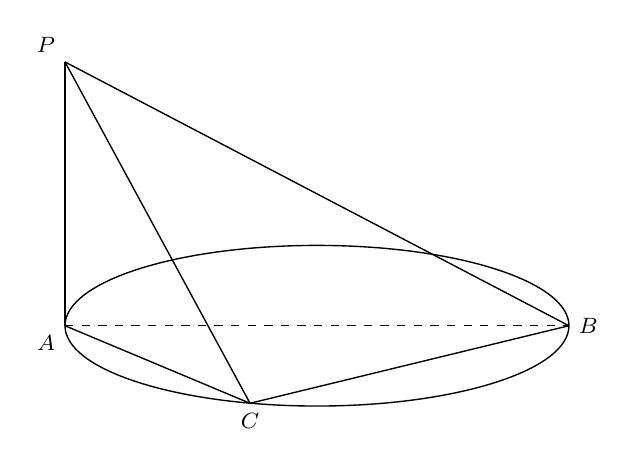
\begin{tikzpicture}[font=\footnotesize, line width=0.5pt, scale=1]
  \coordinate (A) at (-3.2,0);
  \coordinate (B) at (3.2,0);
  \coordinate (C) at (-0.85,-0.985);
  \coordinate (P) at (-3.2,3.35);
  % 底面圆（斜二测画法下的椭圆）
  \draw (0,0) ellipse (3.2 and 1.02);
  % 可见棱
  \draw (P) -- (A);
  \draw (P) -- (B);
  \draw (P) -- (C);
  \draw (A) -- (C);
  \draw (C) -- (B);
  % 被遮挡的直径
  \draw[dashed] (A) -- (B);
  % 点与标签
  \node[above left] at (P) {$P$};
  \node[below left] at (A) {$A$};
  \node[right] at (B) {$B$};
  \node[below] at (C) {$C$};
\end{tikzpicture}
\end{center}
\nopagebreak[4]
\Needspace{4\baselineskip}
\textbf{解析}
\Needspace{5\baselineskip}
\textbf{（1）} 因为 $AB$ 是圆的直径，$C$ 在圆上，由直径所对的圆周角为直角得
\nopagebreak[4]
\[BC\perp AC.\]
\Needspace{5\baselineskip}
又 $PA\perp$ 圆所在的平面，而 $BC$ 在该平面内，所以
\nopagebreak[4]
\[PA\perp BC.\]
\Needspace{5\baselineskip}
$PA$，$AC$ 是平面 $PAC$ 内两条相交直线，故
\nopagebreak[4]
\[BC\perp\text{\text{平面} }PAC.\]
\Needspace{5\baselineskip}
又 $BC\subset$ 平面 $PBC$，所以
\nopagebreak[4]
\[\text{\text{平面} }PAC\perp\text{\text{平面} }PBC.\]

\Needspace{5\baselineskip}
\textbf{（2）} 以 $O$ 为原点，$AB$ 所在直线为 $x$ 轴，圆所在平面为 $xOy$ 平面建立空间直角坐标系。由 $AB=2$ 可取
\nopagebreak[4]
\[A(-1,0,0),\qquad B(1,0,0).\]
\Needspace{5\baselineskip}
设 $C(x,y,0)$。由 $C$ 在圆上及 $AC=1$，
\nopagebreak[4]
\[\begin{cases}x^2+y^2=1,\\(x+1)^2+y^2=1.\end{cases}\]
\Needspace{5\baselineskip}
两式相减得 $2x+1=0$，即 $x=-\dfrac12$，进而 $y=\dfrac{\sqrt3}2$（取上半圆，不影响夹角）。故
\nopagebreak[4]
\[C\left(-\frac12,\frac{\sqrt3}2,0\right).\]
\Needspace{5\baselineskip}
又 $PA=1$ 且 $PA\perp$ 圆面，故
\nopagebreak[4]
\[P(-1,0,1).\]
\Needspace{5\baselineskip}
于是
\nopagebreak[4]
\[\overrightarrow{PB}=(2,0,-1),\qquad
\overrightarrow{PC}=\left(\frac12,\frac{\sqrt3}2,-1\right),\qquad
\overrightarrow{PA}=(0,0,-1).\]
\Needspace{5\baselineskip}
平面 $PBC$ 的一个法向量为
\nopagebreak[4]
\[\boldsymbol n_1=\overrightarrow{PB}\times\overrightarrow{PC}
=\left(\frac{\sqrt3}2,\frac32,\sqrt3\right),\]
\Needspace{5\baselineskip}
平面 $PAB$ 的一个法向量为
\nopagebreak[4]
\[\boldsymbol n_2=(0,1,0).\]
\Needspace{5\baselineskip}
因为二面角 $C-PB-A$ 的平面角为锐角，所以
\nopagebreak[4]
\[\cos\theta=\frac{|\boldsymbol n_1\cdot\boldsymbol n_2|}{|\boldsymbol n_1||\boldsymbol n_2|}
=\frac{\frac32}{\sqrt{\frac34+\frac94+3}\cdot1}
=\frac{\frac32}{\sqrt6}
=\frac{\sqrt6}4.\]
故二面角 $C-PB-A$ 的余弦值为 $\dfrac{\sqrt6}4$。

\gkanswer{答案（1）：证明见解析。由直径所对圆周角为直角得 $BC\perp AC$，又 $PA\perp BC$，故 $BC\perp$ 平面 $PAC$，从而平面 $PBC\perp$ 平面 $PAC$。}

\gkanswer{答案（2）：$\dfrac{\sqrt6}4$。建立空间直角坐标系，两半平面的法向量可取 $\left(\dfrac{\sqrt3}2,\dfrac32,\sqrt3\right)$ 与 $(0,1,0)$，夹角余弦为 $\dfrac{3/2}{\sqrt6}=\dfrac{\sqrt6}4$。}

\end{answer}
\begin{answer}
\gksolhead{19}{}

\textbf{题目}：

现有 $10$ 道题，其中 $6$ 道甲类题，$4$ 道乙类题，张同学从中任取 $3$ 道题解答。

（1） 求张同学至少取到 $1$ 道乙类题的概率；

（2） 已知所取的 $3$ 道题中有 $2$ 道甲类题，$1$ 道乙类题。设张同学答对每道甲类题的概率都是 $\dfrac35$，答对每道乙类题的概率都是 $\dfrac45$，且各题答对与否相互独立。用 $X$ 表示张同学答对题的个数，求 $X$ 的分布列和数学期望。

\Needspace{4\baselineskip}
\textbf{解析}
\Needspace{5\baselineskip}
\textbf{（1）} 从 $10$ 道题中任取 $3$ 道，共有 $\mathrm C_{10}^3$ 种等可能取法。“至少取到 $1$ 道乙类题”的对立事件是“取到的 $3$ 道全是甲类题”，其取法数为 $\mathrm C_6^3$。故所求概率为
\nopagebreak[4]
\[P=1-\frac{\mathrm C_6^3}{\mathrm C_{10}^3}
=1-\frac{20}{120}
=\frac56.\]

\Needspace{5\baselineskip}
\textbf{（2）} 已知取到的 $3$ 道题中有 $2$ 道甲类题、$1$ 道乙类题。设答对甲类题的个数为 $X_1$，答对乙类题的个数为 $X_2$，则
\nopagebreak[4]
\[X_1\sim B\left(2,\frac35\right),\qquad X_2\sim B\left(1,\frac45\right),\]
且 $X=X_1+X_2$，$X_1$ 与 $X_2$ 相互独立。

\Needspace{5\baselineskip}
分别计算：
\nopagebreak[4]
\[P(X=0)=\left(\frac25\right)^2\cdot\frac15=\frac4{125};\]
\nopagebreak[4]
\[\begin{aligned}
P(X=1)&=\mathrm C_2^1\cdot\frac35\cdot\frac25\cdot\frac15+\left(\frac25\right)^2\cdot\frac45\\
&=\frac{12}{125}+\frac{16}{125}=\frac{28}{125};
\end{aligned}\]
\nopagebreak[4]
\[\begin{aligned}
P(X=2)&=\left(\frac35\right)^2\cdot\frac15+\mathrm C_2^1\cdot\frac35\cdot\frac25\cdot\frac45\\
&=\frac9{125}+\frac{48}{125}=\frac{57}{125};
\end{aligned}\]
\nopagebreak[4]
\[P(X=3)=\left(\frac35\right)^2\cdot\frac45=\frac{36}{125}.\]
所以 $X$ 的分布列为

\begin{center}
\begin{tabular}{lllll}
\toprule
$X$ & $0$ & $1$ & $2$ & $3$ \\
\midrule
$P$ & $\dfrac4{125}$ & $\dfrac{28}{125}$ & $\dfrac{57}{125}$ & $\dfrac{36}{125}$ \\
\bottomrule
\end{tabular}
\end{center}

\Needspace{5\baselineskip}
数学期望为
\nopagebreak[4]
\[\begin{aligned}
E(X)&=0\cdot\frac4{125}+1\cdot\frac{28}{125}+2\cdot\frac{57}{125}+3\cdot\frac{36}{125}\\
&=\frac{28+114+108}{125}
=\frac{250}{125}=2.
\end{aligned}\]
\Needspace{5\baselineskip}
也可由期望的线性性质直接得
\nopagebreak[4]
\[E(X)=2\cdot\frac35+1\cdot\frac45=2.\]

\gkanswer{答案（1）：$\dfrac56$。$1-\dfrac{\mathrm C_6^3}{\mathrm C_{10}^3}=1-\dfrac{20}{120}=\dfrac56$。}

\gkanswer{答案（2）：$P(X=0)=\dfrac4{125}$，$P(X=1)=\dfrac{28}{125}$，$P(X=2)=\dfrac{57}{125}$，$P(X=3)=\dfrac{36}{125}$，$E(X)=2$。}

\end{answer}
\begin{answer}
\gksolhead{20}{}

\textbf{题目}：

如图，抛物线 $C_1:x^2=4y$，$C_2:x^2=-2py$（$p>0$）。点 $M(x_0,y_0)$ 在抛物线 $C_2$ 上，过 $M$ 作 $C_1$ 的切线，切点为 $A$，$B$（$M$ 为原点 $O$ 时，$A$，$B$ 重合于 $O$）。当 $x_0=1-\sqrt2$ 时，切线 $MA$ 的斜率为 $-\dfrac12$。

（1） 求 $p$ 的值；

（2） 当 $M$ 在 $C_2$ 上运动时，求线段 $AB$ 中点 $N$ 的轨迹方程（$A$，$B$ 重合于 $O$ 时，中点为 $O$）。
\nopagebreak[4]
\begin{center}% 2013 年辽宁卷理科第 20 题：抛物线 C1、C2 与过 M 的两条切线。
% 来源 PDF：普通高考/2013/2013辽宁理.pdf，第 2 页（印面 822）左栏。
% 由第（1）问得 p=2，故图中 C2 为 x^2=-4y。
\begin{tikzpicture}[font=\footnotesize, line width=0.5pt, >=Stealth, scale=1.15]
  % 坐标轴
  \draw[->] (-3.3,0) -- (3.5,0) node[below] {$x$};
  \draw[->] (0,-2.8) -- (0,2.9) node[right] {$y$};
  \node[below right] at (0,0) {$O$};
  % C1: x^2=4y, 即 y=x^2/4
  \draw[domain=-3.15:3.15, smooth, samples=120] plot (\x,{\x*\x/4});
  % C2: x^2=-4y, 即 y=-x^2/4
  \draw[domain=-3.15:3.15, smooth, samples=120] plot (\x,{-\x*\x/4});
  % M(-1,-0.25) 在 C2 上；两条切线的切点
  \coordinate (M) at (-1,-0.25);
  \coordinate (A) at (-2.4142,1.4572);
  \coordinate (B) at (0.4142,0.0429);
  \draw ($(M)!-0.25!(A)$) -- ($(M)!1.22!(A)$);
  \draw ($(M)!-0.25!(B)$) -- ($(M)!1.55!(B)$);
  \fill (M) circle (1.4pt) node[below right] {$M$};
  \node[above] at (A) {$A$};
  \node[above right] at (B) {$B$};
\end{tikzpicture}
\end{center}
\nopagebreak[4]
\Needspace{4\baselineskip}
\textbf{解析}
\Needspace{5\baselineskip}
\textbf{（1）} 设切点 $A\left(t,\dfrac{t^2}4\right)$。由 $y=\dfrac{x^2}4$ 得 $y'=\dfrac x2$，故 $C_1$ 在 $A$ 处的切线为
\nopagebreak[4]
\[y=\frac t2x-\frac{t^2}4.\]
\Needspace{5\baselineskip}
它过 $M(x_0,y_0)$，代入得
\nopagebreak[4]
\[y_0=\frac t2x_0-\frac{t^2}4,\]
\Needspace{5\baselineskip}
即
\nopagebreak[4]
\[t^2-2x_0t+4y_0=0. \tag{①}\]
两条切线的切点对应的参数 $t_1$，$t_2$ 是方程①的两根，且切线斜率分别为 $\dfrac{t_1}2$，$\dfrac{t_2}2$。

\Needspace{5\baselineskip}
已知切线 $MA$ 的斜率为 $-\dfrac12$，故 $t_1=-1$。将 $t=-1$ 代入①：
\nopagebreak[4]
\[1+2x_0+4y_0=0.\]
\Needspace{5\baselineskip}
由 $x_0=1-\sqrt2$ 得
\nopagebreak[4]
\[4y_0=-1-2(1-\sqrt2)=2\sqrt2-3,\]
\Needspace{5\baselineskip}
即
\nopagebreak[4]
\[y_0=\frac{2\sqrt2-3}4.\]
\Needspace{5\baselineskip}
又 $M$ 在 $C_2:x^2=-2py$ 上，故
\nopagebreak[4]
\[(1-\sqrt2)^2=-2p\cdot\frac{2\sqrt2-3}4.\]
\Needspace{5\baselineskip}
左边
\nopagebreak[4]
\[(1-\sqrt2)^2=3-2\sqrt2,\]
\Needspace{5\baselineskip}
右边
\nopagebreak[4]
\[-2p\cdot\frac{2\sqrt2-3}4=\frac{p(3-2\sqrt2)}2.\]
\Needspace{5\baselineskip}
因为 $3-2\sqrt2\neq0$，所以
\nopagebreak[4]
\[\frac p2=1,\]
\Needspace{5\baselineskip}
即
\nopagebreak[4]
\[p=2.\]

\Needspace{5\baselineskip}
\textbf{（2）} 设 $A$，$B$ 对应的参数为 $t_1$，$t_2$。由①及韦达定理，
\nopagebreak[4]
\[t_1+t_2=2x_0,\qquad t_1t_2=4y_0.\]
\Needspace{5\baselineskip}
线段 $AB$ 的中点 $N(x,y)$ 满足
\nopagebreak[4]
\[x=\frac{t_1+t_2}2=x_0,\]
\nopagebreak[4]
\[\begin{aligned}
y&=\frac18\left(t_1^2+t_2^2\right)
=\frac18\left[(t_1+t_2)^2-2t_1t_2\right]\\
&=\frac{4x_0^2-8y_0}8
=\frac{x_0^2-2y_0}2.
\end{aligned}\]
\Needspace{5\baselineskip}
由（1）知 $p=2$，即 $C_2:x^2=-4y$，故
\nopagebreak[4]
\[y_0=-\frac{x_0^2}4.\]
\Needspace{5\baselineskip}
代入得
\nopagebreak[4]
\[y=\frac{x_0^2+\dfrac{x_0^2}2}2=\frac34x_0^2.\]
\Needspace{5\baselineskip}
又 $x=x_0$，所以
\nopagebreak[4]
\[y=\frac34x^2,\quad\text{\text{即}}\quad x^2=\frac43y.\]

\Needspace{5\baselineskip}
反之，对任意实数 $x_0$，取 $M\left(x_0,-\dfrac{x_0^2}4\right)\in C_2$，方程①的判别式
\nopagebreak[4]
\[\Delta=4x_0^2-16y_0=4x_0^2+4x_0^2=8x_0^2\geqslant0,\]
\Needspace{5\baselineskip}
两条切线存在（$x_0=0$ 时重合于 $O$），对应中点
\nopagebreak[4]
\[N\left(x_0,\frac34x_0^2\right).\]
\Needspace{5\baselineskip}
故所求轨迹方程为
\nopagebreak[4]
\[y=\frac34x^2\quad(x\in\mathbf R).\]

\gkanswer{答案（1）：$p=2$。切线斜率给出切点参数 $t=-1$，代入 $t^2-2x_0t+4y_0=0$ 并与 $C_2$ 联立，得 $p=2$。}

\gkanswer{答案（2）：$y=\dfrac34x^2$（$x\in\mathbf R$）。设切点参数 $t_1$，$t_2$，则 $x=x_0$，$y=\dfrac{x_0^2-2y_0}2$；用 $y_0=-\dfrac{x_0^2}4$ 消去 $y_0$ 即得。}

\end{answer}
\begin{answer}
\gksolhead{21}{}

\textbf{题目}：

已知函数 $f(x)=(1+x)\mathrm e^{-2x}$，$g(x)=ax+\dfrac{x^3}2+1+2x\cos x$，当 $x\in[0,1]$ 时，

（1） 求证：$1-x\leqslant f(x)\leqslant\dfrac1{1+x}$；

（2） 若 $f(x)\geqslant g(x)$ 恒成立，求实数 $a$ 的取值范围。

\Needspace{4\baselineskip}
\textbf{解析}
\Needspace{5\baselineskip}
\textbf{（1）} 先证下界。令
\nopagebreak[4]
\[h(x)=f(x)-(1-x)=(1+x)\mathrm e^{-2x}-1+x,\qquad x\in[0,1].\]
\Needspace{5\baselineskip}
则 $h(0)=0$，且
\nopagebreak[4]
\[h'(x)=1-(1+2x)\mathrm e^{-2x},\qquad h'(0)=0.\]
\Needspace{5\baselineskip}
再求导：
\nopagebreak[4]
\[h''(x)=4x\mathrm e^{-2x}\geqslant0\qquad(x\geqslant0).\]
\Needspace{5\baselineskip}
所以 $h'$ 在 $[0,1]$ 上单调递增，从而
\nopagebreak[4]
\[h'(x)\geqslant h'(0)=0.\]
\Needspace{5\baselineskip}
于是 $h$ 在 $[0,1]$ 上单调递增，
\nopagebreak[4]
\[h(x)\geqslant h(0)=0,\]
\Needspace{5\baselineskip}
即
\nopagebreak[4]
\[f(x)\geqslant1-x.\]

\Needspace{5\baselineskip}
再证上界。$f(x)\leqslant\dfrac1{1+x}$ 等价于
\nopagebreak[4]
\[(1+x)^2\mathrm e^{-2x}\leqslant1,\]
\Needspace{5\baselineskip}
两边开平方（均为正）得
\nopagebreak[4]
\[(1+x)\mathrm e^{-x}\leqslant1.\]
\Needspace{5\baselineskip}
令
\nopagebreak[4]
\[\varphi(x)=(1+x)\mathrm e^{-x},\]
\Needspace{5\baselineskip}
则
\nopagebreak[4]
\[\varphi'(x)=\mathrm e^{-x}-(1+x)\mathrm e^{-x}=-x\mathrm e^{-x}\leqslant0,\]
\Needspace{5\baselineskip}
故 $\varphi$ 在 $[0,1]$ 上单调递减，
\nopagebreak[4]
\[\varphi(x)\leqslant\varphi(0)=1.\]
\Needspace{5\baselineskip}
因此
\nopagebreak[4]
\[f(x)\leqslant\frac1{1+x}.\]
\Needspace{5\baselineskip}
综上，
\nopagebreak[4]
\[1-x\leqslant f(x)\leqslant\frac1{1+x}.\]

\Needspace{5\baselineskip}
\textbf{（2）} 令
\nopagebreak[4]
\[u(x)=f(x)-g(x)=(1+x)\mathrm e^{-2x}-ax-\frac{x^3}2-1-2x\cos x.\]
\Needspace{5\baselineskip}
则 $u(0)=0$。若 $u(x)\geqslant0$ 对 $x\in[0,1]$ 恒成立，则
\nopagebreak[4]
\[u'(0)=\lim_{x\to0^+}\frac{u(x)-u(0)}x\geqslant0.\]
\Needspace{5\baselineskip}
而
\nopagebreak[4]
\[u'(x)=-(1+2x)\mathrm e^{-2x}-a-\frac32x^2-2\cos x+2x\sin x,\]
\Needspace{5\baselineskip}
故
\nopagebreak[4]
\[u'(0)=-1-a-2=-(a+3).\]
\Needspace{5\baselineskip}
于是
\nopagebreak[4]
\[-(a+3)\geqslant0,\]
\Needspace{5\baselineskip}
即
\nopagebreak[4]
\[a\leqslant-3.\]
这说明 $a\leqslant-3$ 是必要条件。

\Needspace{5\baselineskip}
下面证明充分性。当 $a\leqslant-3$ 时，对 $x\in[0,1]$，
\nopagebreak[4]
\[g(x)=ax+\frac{x^3}2+1+2x\cos x
\leqslant-3x+\frac{x^3}2+1+2x\cos x=:g_{-3}(x).\]
\Needspace{5\baselineskip}
因此只需证明
\nopagebreak[4]
\[f(x)\geqslant g_{-3}(x).\]
\Needspace{5\baselineskip}
由（1）知 $f(x)\geqslant1-x$，故只需证明
\nopagebreak[4]
\[1-x\geqslant g_{-3}(x),\]
\Needspace{5\baselineskip}
即
\nopagebreak[4]
\[1-x\geqslant-3x+\frac{x^3}2+1+2x\cos x.\]
\Needspace{5\baselineskip}
移项得
\nopagebreak[4]
\[2x-\frac{x^3}2-2x\cos x\geqslant0,\]
\Needspace{5\baselineskip}
即
\nopagebreak[4]
\[x\left(2-2\cos x-\frac{x^2}2\right)\geqslant0.\]
\Needspace{5\baselineskip}
当 $x=0$ 时等号成立。当 $0<x\leqslant1$ 时，只需证
\nopagebreak[4]
\[2-2\cos x\geqslant\frac{x^2}2.\]
\Needspace{5\baselineskip}
令
\nopagebreak[4]
\[q(x)=1-\cos x-\frac{x^2}4,\]
\Needspace{5\baselineskip}
则 $q(0)=0$，且
\nopagebreak[4]
\[q'(x)=\sin x-\frac x2.\]
\Needspace{5\baselineskip}
因为 $\dfrac{\sin x}{x}$ 在 $(0,1]$ 上单调递减，且
\nopagebreak[4]
\[\sin1>\sin\frac{\pi}6=\frac12\]
\Needspace{5\baselineskip}
（这里 $1>\dfrac{\pi}6$），所以
\nopagebreak[4]
\[\frac{\sin x}{x}\geqslant\sin1>\frac12,\]
\Needspace{5\baselineskip}
即 $\sin x>\dfrac x2$。于是 $q'(x)>0$，$q$ 在 $[0,1]$ 上单调递增，
\nopagebreak[4]
\[q(x)\geqslant q(0)=0,\]
\Needspace{5\baselineskip}
从而
\nopagebreak[4]
\[1-\cos x\geqslant\frac{x^2}4,\]
\Needspace{5\baselineskip}
即
\nopagebreak[4]
\[2-2\cos x\geqslant\frac{x^2}2.\]
\Needspace{5\baselineskip}
因此
\nopagebreak[4]
\[g_{-3}(x)\leqslant1-x\leqslant f(x).\]
所以当 $a\leqslant-3$ 时，$f(x)\geqslant g(x)$ 恒成立。

\Needspace{5\baselineskip}
综上，实数 $a$ 的取值范围为
\nopagebreak[4]
\[a\leqslant-3.\]

\gkanswer{答案（1）：证明见解析。令 $h=f-(1-x)$，由 $h''(x)=4x\mathrm e^{-2x}\geqslant0$ 及 $h(0)=h'(0)=0$ 得下界；上界等价于 $(1+x)\mathrm e^{-x}\leqslant1$。}

\gkanswer{答案（2）：$a\leqslant-3$。必要性由 $x=0$ 处 $f-g$ 的右导数 $-(a+3)\geqslant0$ 得出；充分性用 $a\leqslant-3$ 时 $g_a(x)\leqslant g_{-3}(x)$，并验证 $g_{-3}(x)\leqslant1-x\leqslant f(x)$。}

\end{answer}
\begin{answer}
\gksolhead{22}{}

\textbf{题目}：

如图，$AB$ 为 $\odot O$ 直径，直线 $CD$ 与 $\odot O$ 相切于 $E$，$AD$ 垂直 $CD$ 于 $D$，$BC$ 垂直 $CD$ 于 $C$，$EF$ 垂直 $AB$ 于 $F$，连接 $AE$，$BE$。证明：

（1） $\angle FEB=\angle CEB$；

（2） $EF^2=AD\cdot BC$。
\nopagebreak[4]
\begin{center}% 2013 年辽宁卷理科第 22 题：AB 为 ⊙O 直径，CD 切 ⊙O 于 E，
% AD⊥CD，BC⊥CD，EF⊥AB。
% 来源 PDF：普通高考/2013/2013辽宁理.pdf，第 2 页（印面 822）中栏。
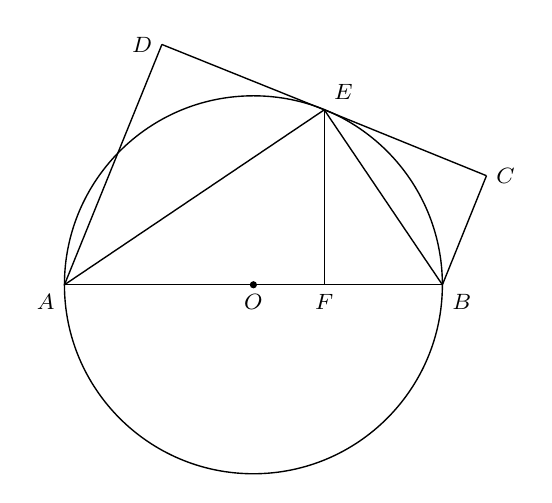
\begin{tikzpicture}[font=\footnotesize, line width=0.5pt, scale=1.0]
  \coordinate (O) at (0,0);
  \coordinate (A) at (-2.4,0);
  \coordinate (B) at (2.4,0);
  \coordinate (E) at (0.90,2.222);
  \coordinate (F) at (0.90,0);
  \coordinate (D) at (-1.162,3.052);
  \coordinate (C) at (2.960,1.385);
  % 圆
  \draw (O) circle (2.4);
  % 直径与切线
  \draw (A) -- (B);
  \draw (D) -- (E) -- (C);
  % 垂线
  \draw (A) -- (D);
  \draw (B) -- (C);
  \draw (E) -- (F);
  % 连接 AE、BE
  \draw (A) -- (E);
  \draw (B) -- (E);
  % 点与标签
  \fill (O) circle (1.3pt) node[below] {$O$};
  \node[below left] at (A) {$A$};
  \node[below right] at (B) {$B$};
  \node[above right] at (E) {$E$};
  \node[left] at (D) {$D$};
  \node[right] at (C) {$C$};
  \node[below] at (F) {$F$};
\end{tikzpicture}
\end{center}
\nopagebreak[4]
\Needspace{4\baselineskip}
\textbf{解析}
\Needspace{5\baselineskip}
\textbf{（1）} 因为 $CD$ 与 $\odot O$ 相切于 $E$，由弦切角定理，
\nopagebreak[4]
\[\angle CEB=\angle EAB.\]
\Needspace{5\baselineskip}
又 $AB$ 为直径，故
\nopagebreak[4]
\[\angle AEB=90^\circ.\]
\Needspace{5\baselineskip}
因为 $EF\perp AB$，所以在直角三角形 $AEF$ 中，
\nopagebreak[4]
\[\angle AEF=90^\circ-\angle EAF=90^\circ-\angle EAB.\]
\Needspace{5\baselineskip}
于是
\nopagebreak[4]
\[\begin{aligned}
\angle FEB&=\angle AEB-\angle AEF\\
&=90^\circ-\left(90^\circ-\angle EAB\right)\\
&=\angle EAB=\angle CEB.
\end{aligned}\]

\Needspace{5\baselineskip}
\textbf{（2）} 由（1）知 $\angle FEB=\angle CEB$。又
\nopagebreak[4]
\[\angle EFB=\angle ECB=90^\circ,\]
\Needspace{5\baselineskip}
且 $EB$ 为公共边，故
\nopagebreak[4]
\[\triangle EFB\cong\triangle ECB,\]
\Needspace{5\baselineskip}
从而
\nopagebreak[4]
\[EF=EC,\qquad BF=BC.\]

\Needspace{5\baselineskip}
同理，由弦切角定理，
\nopagebreak[4]
\[\angle DEA=\angle EBA.\]
\Needspace{5\baselineskip}
而
\nopagebreak[4]
\[\angle FEA=90^\circ-\angle FEB=90^\circ-\angle EAB=\angle EBA,\]
\Needspace{5\baselineskip}
故
\nopagebreak[4]
\[\angle FEA=\angle DEA.\]
\Needspace{5\baselineskip}
又
\nopagebreak[4]
\[\angle EFA=\angle EDA=90^\circ,\]
\Needspace{5\baselineskip}
且 $EA$ 为公共边，故
\nopagebreak[4]
\[\triangle EFA\cong\triangle EDA,\]
\Needspace{5\baselineskip}
从而
\nopagebreak[4]
\[EF=ED,\qquad AF=AD.\]

\Needspace{5\baselineskip}
于是
\nopagebreak[4]
\[AD\cdot BC=AF\cdot BF.\]
\Needspace{5\baselineskip}
在直角三角形 $AEB$ 中，$EF$ 是斜边 $AB$ 上的高，由射影定理，
\nopagebreak[4]
\[EF^2=AF\cdot BF.\]
\Needspace{5\baselineskip}
所以
\nopagebreak[4]
\[EF^2=AD\cdot BC.\]

\gkanswer{答案（1）：证明见解析。切线弦定理给 $\angle CEB=\angle EAB$，再由 $AB$ 为直径及 $EF\perp AB$ 得 $\angle FEB=\angle EAB$。}

\gkanswer{答案（2）：证明见解析。由（1）可证 $\triangle EFB\cong\triangle ECB$，$\triangle EFA\cong\triangle EDA$，故 $AD=AF$，$BC=BF$；再由直角三角形 $AEB$ 的射影定理 $EF^2=AF\cdot BF$。}

\end{answer}
\begin{answer}
\gksolhead{23}{}

\textbf{题目}：

在直角坐标系 $xOy$ 中，以 $O$ 为极点，$x$ 轴正半轴为极轴建立极坐标系。圆 $C_1$、直线 $C_2$ 的极坐标方程分别为 $\rho=4\sin\theta$，$\rho\cos\left(\theta-\dfrac{\pi}4\right)=2\sqrt2$。

（1） 求 $C_1$ 与 $C_2$ 交点的极坐标；

\Needspace{5\baselineskip}
（2） 设 $P$ 为 $C_1$ 的圆心，$Q$ 为 $C_1$ 与 $C_2$ 交点连线的中点，已知直线 $PQ$ 的参数方程为
\nopagebreak[4]
\[\begin{cases}x=t^3+a,\\[2pt] y=\dfrac b2t^3+1,\end{cases}\quad(t\in\mathbf R\ \text{\text{为参数}})\]
求 $a$，$b$ 的值。

\Needspace{4\baselineskip}
\textbf{解析}
\Needspace{5\baselineskip}
\textbf{（1）} 由 $\rho=4\sin\theta$ 得
\nopagebreak[4]
\[\rho^2=4\rho\sin\theta,\]
\Needspace{5\baselineskip}
即
\nopagebreak[4]
\[x^2+y^2=4y,\]
\Needspace{5\baselineskip}
配方得
\nopagebreak[4]
\[x^2+(y-2)^2=4.\]
所以 $C_1$ 是以 $(0,2)$ 为圆心、$2$ 为半径的圆。

\Needspace{5\baselineskip}
由 $\rho\cos\left(\theta-\dfrac{\pi}4\right)=2\sqrt2$ 得
\nopagebreak[4]
\[\frac{\sqrt2}2(\rho\cos\theta+\rho\sin\theta)=2\sqrt2,\]
\Needspace{5\baselineskip}
即
\nopagebreak[4]
\[x+y=4.\]
所以 $C_2$ 是直线 $x+y=4$。

\Needspace{5\baselineskip}
将 $y=4-x$ 代入 $x^2+y^2=4y$：
\nopagebreak[4]
\[x^2+(4-x)^2=4(4-x),\]
\Needspace{5\baselineskip}
展开得
\nopagebreak[4]
\[2x^2-8x+16=16-4x,\]
\Needspace{5\baselineskip}
即
\nopagebreak[4]
\[2x^2-4x=0,\]
\nopagebreak[4]
\[2x(x-2)=0.\]
\Needspace{5\baselineskip}
所以 $x=0$ 或 $x=2$，对应交点为
\nopagebreak[4]
\[(0,4),\qquad(2,2).\]
\Needspace{5\baselineskip}
化为极坐标：
\nopagebreak[4]
\[(0,4)\longleftrightarrow\left(4,\frac{\pi}2\right),\qquad
(2,2)\longleftrightarrow\left(2\sqrt2,\frac{\pi}4\right).\]
\Needspace{5\baselineskip}
故交点的极坐标为
\nopagebreak[4]
\[\left(4,\frac{\pi}2\right),\qquad\left(2\sqrt2,\frac{\pi}4\right).\]

\Needspace{5\baselineskip}
\textbf{（2）} 由（1）知 $C_1$ 的圆心
\nopagebreak[4]
\[P(0,2).\]
\Needspace{5\baselineskip}
两交点 $(0,4)$，$(2,2)$ 连线的中点为
\nopagebreak[4]
\[Q\left(\frac{0+2}2,\frac{4+2}2\right)=(1,3).\]
\Needspace{5\baselineskip}
直线 $PQ$ 的斜率为
\nopagebreak[4]
\[k=\frac{3-2}{1-0}=1,\]
\Needspace{5\baselineskip}
故其方程为
\nopagebreak[4]
\[y-2=1\cdot(x-0),\]
\Needspace{5\baselineskip}
即
\nopagebreak[4]
\[y=x+2.\]

\Needspace{5\baselineskip}
已知参数方程
\nopagebreak[4]
\[\begin{cases}x=t^3+a,\\ y=\dfrac b2t^3+1.\end{cases}\]
\Needspace{5\baselineskip}
消去 $t^3$ 得
\nopagebreak[4]
\[y=\frac b2(x-a)+1
=\frac b2x+1-\frac{ab}2.\]
\Needspace{5\baselineskip}
与 $y=x+2$ 比较系数：
\nopagebreak[4]
\[\frac b2=1,\qquad 1-\frac{ab}2=2.\]
\Needspace{5\baselineskip}
由第一式得 $b=2$，代入第二式：
\nopagebreak[4]
\[1-a=2,\]
\Needspace{5\baselineskip}
故
\nopagebreak[4]
\[a=-1.\]
\Needspace{5\baselineskip}
所以
\nopagebreak[4]
\[a=-1,\qquad b=2.\]

\gkanswer{答案（1）：$(4,\dfrac{\pi}2)$，$(2\sqrt2,\dfrac{\pi}4)$。$C_1$ 为 $x^2+(y-2)^2=4$，$C_2$ 为 $x+y=4$，交点为 $(0,4)$，$(2,2)$。}

\gkanswer{答案（2）：$a=-1$，$b=2$。$P(0,2)$，$Q(1,3)$，直线 $PQ$ 为 $y=x+2$；与参数方程比较斜率和截距即得。}

\end{answer}
\begin{answer}
\gksolhead{24}{}

\textbf{题目}：

已知函数 $f(x)=|x-a|$，其中 $a>1$。

（1） 当 $a=2$ 时，求不等式 $f(x)\geqslant4-|x-4|$ 的解集；

（2） 已知关于 $x$ 的不等式 $|f(2x+a)-2f(x)|\leqslant2$ 的解集为 $\{x\mid1\leqslant x\leqslant2\}$，求 $a$ 的值。

\Needspace{4\baselineskip}
\textbf{解析}
\Needspace{5\baselineskip}
\textbf{（1）} 当 $a=2$ 时，
\nopagebreak[4]
\[f(x)=|x-2|,\]
\Needspace{5\baselineskip}
不等式为
\nopagebreak[4]
\[|x-2|\geqslant4-|x-4|.\]
按零点 $2$，$4$ 分段讨论。

\Needspace{5\baselineskip}
当 $x<2$ 时，$|x-2|=2-x$，$|x-4|=4-x$，不等式化为
\nopagebreak[4]
\[2-x\geqslant4-(4-x)=x,\]
\Needspace{5\baselineskip}
即
\nopagebreak[4]
\[2\geqslant2x,\]
\nopagebreak[4]
\[x\leqslant1.\]
结合 $x<2$，得 $x\leqslant1$。

\Needspace{5\baselineskip}
当 $2\leqslant x\leqslant4$ 时，$|x-2|=x-2$，$|x-4|=4-x$，不等式化为
\nopagebreak[4]
\[x-2\geqslant4-(4-x)=x,\]
\Needspace{5\baselineskip}
即
\nopagebreak[4]
\[-2\geqslant0,\]
无解。

\Needspace{5\baselineskip}
当 $x>4$ 时，$|x-2|=x-2$，$|x-4|=x-4$，不等式化为
\nopagebreak[4]
\[x-2\geqslant4-(x-4)=8-x,\]
\Needspace{5\baselineskip}
即
\nopagebreak[4]
\[2x\geqslant10,\]
\nopagebreak[4]
\[x\geqslant5.\]
结合 $x>4$，得 $x\geqslant5$。

\Needspace{5\baselineskip}
综上，解集为
\nopagebreak[4]
\[(-\infty,1]\cup[5,+\infty).\]

\Needspace{5\baselineskip}
\textbf{（2）} 因为
\nopagebreak[4]
\[f(2x+a)=|(2x+a)-a|=|2x|=2|x|,\]
\nopagebreak[4]
\[2f(x)=2|x-a|,\]
\Needspace{5\baselineskip}
所以原不等式化为
\nopagebreak[4]
\[\bigl|2|x|-2|x-a|\bigr|\leqslant2,\]
\Needspace{5\baselineskip}
即
\nopagebreak[4]
\[\bigl||x|-|x-a|\bigr|\leqslant1.\]

因为 $a>1$，分三段讨论：

\begin{itemize}
\item 当 $x\leqslant0$ 时，$|x|=-x$，$|x-a|=a-x$，故
\end{itemize}
\nopagebreak[4]
\[\bigl||x|-|x-a|\bigr|=|-x-(a-x)|=a>1,\]
不满足不等式；
\begin{itemize}
\item 当 $0\leqslant x\leqslant a$ 时，$|x|=x$，$|x-a|=a-x$，故
\end{itemize}
\nopagebreak[4]
\[\bigl||x|-|x-a|\bigr|=|x-(a-x)|=|2x-a|,\]
\Needspace{5\baselineskip}
不等式化为
\nopagebreak[4]
\[|2x-a|\leqslant1,\]
\Needspace{5\baselineskip}
即
\nopagebreak[4]
\[-1\leqslant2x-a\leqslant1,\]
\nopagebreak[4]
\[\frac{a-1}2\leqslant x\leqslant\frac{a+1}2;\]
\begin{itemize}
\item 当 $x\geqslant a$ 时，$|x|=x$，$|x-a|=x-a$，故
\end{itemize}
\nopagebreak[4]
\[\bigl||x|-|x-a|\bigr|=|x-(x-a)|=a>1,\]
不满足不等式。

\Needspace{5\baselineskip}
因此原不等式的解集为
\nopagebreak[4]
\[\left[\frac{a-1}2,\frac{a+1}2\right].\]
\Needspace{5\baselineskip}
已知解集为 $[1,2]$，故
\nopagebreak[4]
\[\frac{a-1}2=1,\qquad\frac{a+1}2=2.\]
\Needspace{5\baselineskip}
两式均给出
\nopagebreak[4]
\[a=3.\]
\Needspace{5\baselineskip}
所以
\nopagebreak[4]
\[a=3.\]

\gkanswer{答案（1）：$(-\infty,1]\cup[5,+\infty)$。按 $x<2$，$2\leqslant x\leqslant4$，$x>4$ 三段去掉绝对值求解。}

\gkanswer{答案（2）：$a=3$。不等式化为 $\bigl||x|-|x-a|\bigr|\leqslant1$，因 $a>1$，解集为 $\left[\dfrac{a-1}2,\dfrac{a+1}2\right]$，与 $[1,2]$ 比较得 $a=3$。}

\end{answer}